\documentclass[xcolor=dvipsnames]{beamer}
\usepackage{pgf}
\usepackage{tikz}
\usepackage{amsmath,amssymb}
\usepackage{pifont}
\usepackage[latin1]{inputenc}
\usepackage{colortbl}
\usepackage[english]{babel}
\usepackage{comment}
\usepackage{soul}
\usepackage{xspace}
\usepackage{hyperref}
\usepackage{booktabs}        % professional-quality tables
\usepackage{multirow}
\usepackage{standalone}

\usepackage{grffile}
\usepackage{upgreek}
\newcommand{\bmmax}{0} % to fix bold greek fonts
\usepackage{bm}
\usepackage[noend,noline,ruled]{algorithm2e}
\include{mathmacro}


\usetikzlibrary{backgrounds}
\usetikzlibrary{arrows,shapes}
\usetikzlibrary{automata}
\usetikzlibrary{positioning}
\usetikzlibrary{decorations.pathmorphing}
\usetikzlibrary{intersections}
\usetikzlibrary{calc}
\usetikzlibrary{fit}
\usepackage[skins]{tcolorbox}

\usepackage[framemethod=default]{mdframed}


\makeatletter
\newcommand{\bfgreek}[1]{\bm{\@nameuse{#1}}}
\makeatother


\setbeamercovered{invisible}

\usetheme{Malmoe}
\useoutertheme{infolines}
\usefonttheme[onlymath]{serif}
\setbeamertemplate{footline}{%
    \begin{beamercolorbox}[wd=\paperwidth,ht=2.25ex,dp=1ex,right,
      rightskip=4mm, leftskip=5mm]{section in head/foot}
        \inserttitle\hfill\insertauthor\hfill\insertframenumber%
    \end{beamercolorbox}
}
%\setbeamertemplate{footline}[text line]{Greg
%  Shakhnarovich,~~~~Segmentation/cascades,~~~\insertframenumber / \inserttotalframenumber}
\setbeamertemplate{itemize item}[ball]
\setbeamertemplate{itemize subitem}[circle]
\setbeamertemplate{enumerate item}[square]
\setbeamerfont{itemize/enumerate subbody}{size=\normalsize}
\setbeamertemplate{navigation symbols}[only frame symbol]
\setbeamertemplate{subsection in toc shaded}[default][60]

\setbeamertemplate{frametitle}
{
\begin{centering}
\color{black}
\textbf{\insertframetitle}
\par
\end{centering}
}
\setbeamercolor{normal text}{fg=blue!50!black}
\setbeamercolor{math text}{fg=black}
%\setbeamercolor{math text inlined}{use={normal text},fg=normal text.fg}
\setbeamercolor{normal text in math text}{use={normal text},fg=normal text.fg}

\setbeamercolor{bibliography item}{fg=Green}

\usetikzlibrary{shapes,calc,positioning,patterns,decorations.pathmorphing}



\tikzset{cnode/.style={circle,draw,thick,minimum size=2em,inner sep=0pt}}

\tikzset{cnodesmall/.style={circle,draw,thick,minimum size=.5em}}

\colorlet{ffcol}{green!60!black}
\colorlet{bpcol}{red!60!black}



\definecolor{mycolor}{rgb}{0.622, 0.535, 0.698}
\definecolor{superlightgray}{rgb}{0.95, 0.95, 0.93}

\newmdenv[innerlinewidth=4.5pt, roundcorner=24pt,linecolor=mycolor,innerleftmargin=6pt,
innerrightmargin=6pt,innertopmargin=6pt,innerbottommargin=6pt]{linkbox}

\newmdenv[innerlinewidth=0, roundcorner=4pt,backgroundcolor=lightgray,linecolor=mycolor,innerleftmargin=7pt,
innerrightmargin=7pt,innertopmargin=7pt,innerbottommargin=7pt]{codebox}

\newmdenv[innerlinewidth=5pt, roundcorner=4pt,backgroundcolor=superlightgray,linecolor=mycolor,innerleftmargin=5pt,
innerrightmargin=5pt,innertopmargin=5pt,innerbottommargin=5pt]{relatedbox}

\DeclareMathAlphabet{\mathbfsf}{\encodingdefault}{\sfdefault}{bx}{n}


\newcommand{\gt}[1]{col-examples/ctest10k-supp/gt/#1}
\newcommand{\gs}[1]{col-examples/ctest10k-supp/grayscale/#1}
\newcommand{\mm}[1]{col-examples/ctest10k-supp/output/#1}

\newcommand{\cmark}{\ding{51}}
\newcommand{\xmark}{\ding{55}}

\newcommand{\cmt}[1]{\iffalse #1 \fi}
\def\dash{-\phantom{.0}}
\def\ndash{-}
\def\amp{\&} % doesn't screw up table formatting

\def\preli{}
\def\rough{}
\def\guess{}

\def\etal{\emph{et al.}}


\definecolor{cadmiumgreen}{rgb}{0.0, 0.42, 0.24}
\definecolor{deepmagenta}{rgb}{0.8, 0.0, 0.8}
\definecolor{goldenrod}{rgb}{0.85, 0.65, 0.13}

\definecolor{darkgreen}{rgb}{0.0, 0.80, 0.24}


\newcommand{\mycite}[1]{\textcolor{Green}{[{#1}]}}

% TODO: make this directly reference normal text color
\newcommand{\myar}{$\textcolor{blue!50!black}{\Rightarrow}$}

%\date{October 22, 2010}

\colorlet{ffcol}{green!60!black}
\colorlet{bpcol}{red!60!black}


\newcommand{\convarr}[3][ffcol]{% 
% 1: color (default ffcol)
% 2: node label(name)
% 3: distance from node in y
  \foreach \xs in {-.5cm,-.3cm,.5cm} {%
    \draw[{#1},thick,-latex] let \p1 = (#2) in %
    ($ (\x1,\y1)+(\xs,{#3}) $) -- (#2);%
  }%
  \draw let \p1 = (#2) in node at ($ (\x1,\y1)+(0,{#3}) $) {\tiny $\textcolor{#1}{\ldots}$};%
}%

\newcommand{\divarr}[3][ffcol]{% 
% 1: color (default ffcol)
% 2: node label(name)
% 3: distance from node in y
  \foreach \xs in {-.5cm,-.3cm,.5cm} {%
    \draw[{#1},thick,-latex] let \p1 = (#2) in %
    (#2) -- ($ (\x1,\y1)+(\xs,{#3}) $) ;%
  }%
  \draw let \p1 = (#2) in node at ($ (\x1,\y1)+(0,{#3}) $) {\tiny $\textcolor{#1}{\ldots}$};%
}%


\title{Deep Learning Tutorial\\Part I}

\institute{%
  \vspace{-1em}\begin{minipage}[t]{.25\linewidth}%
    \vspace{-3em}%
    \includegraphics[width=.8in]{tticlogo}\vspace{2em}%
  \end{minipage}%
  \begin{minipage}[t]{.5\linewidth}%
    {\Large Greg Shakhnarovich}\\{\Large TTI-Chicago\vspace{2em}}%
  \end{minipage}%
}



\date{December 2016}

\begin{document}

\maketitle

\section{Overview}

\begin{frame}
  \frametitle{Goals of the tutorial}
\bi
\item Somewhat organized overview of basics, and some more advanced
  topics
\item Demistify jargon
\item Pointers for informed further learning
\item Aimed mostly at vision practitioners, but tools are widely
  applicable beyond vision
\item Assumes basic familiarity with machine learning
\ei  
\end{frame}

\begin{frame}
  \frametitle{Not covered}
  \bi
\item Connections to brain
\item Deep learning outside of neural networks
\item Many recent advances
\item Many specialized architectures for vision tasks
\ei
\end{frame}


\begin{frame}
  \frametitle{Outline}
Introduction (3 hours):
\bi
\item Review of relevant machine learning concepts
\item Feedforward neural networks and backpropagation
\item Optimization techniques and issues
\item Complexity and regularization in neural networks
\item Intro to convolutional networks
\ei
Advanced (3 hours):
\bi
\item Advanced techniques for learning DNNs
\item Convnets for tasks beyond image classification
\item Very deep networks
\item Recurrent networks
\ei
\end{frame}

\begin{frame}
  \frametitle{Sources}
  \bi
\item Stanford CS231N: Convolutional Neural Networks for Visual
  Recognition\\
Andrej Karpathy, Justin Johnson et al. (2016 edition)\\
\url{vision.stanford.edu/teaching/cs231n}
\item Deep Learning by Ian Goodfellow, Aaron Courville and Yoshua
  Bengio, 2016
\item Chris Olah: Understanding LSTM Networks (blog post)\\
\url{colah.github.io/posts/2015-08-Understanding-LSTMs}
\item Papers on arXiv and slides by the authors
\ei
\end{frame}


\section{Overview of ML concepts}
\begin{frame}
  \frametitle{Supervised learning: setup}
  \bi
\item Input data space $\mathcal{X}$
\item Output (label, target) space $\mathcal{Y}$\\
image classification: $\mathcal{X} = \{\text{natural images} \}$,\\
$\mathcal{Y}=\{\text{cat},\,\text{dog},\,\text{boat}\,\ldots\}$
\item Unknown function $f:\,\mathcal{X}\,\to\,\mathcal{Y}$
\item Scenario: given a \emph{labeled training set} $(\vx_i,y_i)$,
  $i=1,\ldots,N$, with $\vx_i\in\mathcal{X}$, $y_i\in\mathcal{Y}$.
\item Goal: any for future $\vx$, accurately predict $y$\\
in other words: learn a mapping $f:\,\mathcal{X}\,\to\,\mathcal{Y}$
\ei

\end{frame}


\begin{frame}\frametitle{Loss function}
 \bi
 \item A \emph{loss function}
   $\lf:\,\mathcal{Y}\times\mathcal{Y}\,\to\,\mathbb{R}$ maps
   prediction $\hat{y}$ to
   cost, given true value $y$
 \item Standard choices for regression:\\ 
 squared loss $\lf(\hat{y},y)=(\hat{y}-y)^2$\\
 absolute loss $\lf(\hat{y},y)=|\hat{y}-y|$
\item Standard choice for classification: 0/1 loss
 \[\lf(\hat{y},y)\,=\,
   \begin{cases}
     0 & \text{if}\;y\,=\,\hat{y},\\
     1 & \text{if}\;y\,\ne\,\hat{y},
   \end{cases}
 \]
 or a more general \emph{loss matrix}
 $\mathbf{L}\in\mathbb{R}_{+}^{|\mathcal{Y}|\times|\mathcal{Y}|}$,
 where $\lf(\hat{y},y)\,=\,L_{\hat{y},y}$.
 \ei
 \end{frame}

\begin{frame}\frametitle{Risk of a predictor}
\bi
\item Usually, consider a \emph{parametric} function $f(\vx;\Theta)$\\
E.g., linear function: $f(\vx;\mathbf{w},b)\,=\,\ip{\mathbf{w}}{\mathbf{x}_i}+b$
\item Fundamental assumption:
  example $\vx$/label $y$ are drawn from a joint probability
  distribution $p(\vx,y)$.
\item The ultimate goal is to minimize the \emph{expected loss}, also
  known as \emph{risk}:
\[R(\Theta)\;=\;\Ep{(\vx_0,y_0)\sim p(\vx,y)}{\lf\left(f(\vx_0;\Theta),y_0\right)}\]
\ei



\end{frame}


\begin{frame}\frametitle{Learning by empirical risk minimization} 
\[R(\Theta)\,=\,\Ep{(\vx_0,y_0)\sim p(\vx,y)}{\lf\left(f(\vx_0;\Theta),y_0\right)}\]

\bi
\item Further assumption: data are i.i.d.: same (unknown!) distribution for all pairs $(\vx,y)$
  in both training and test data.
\item Can't find $\argmin_{\Theta}R$, but can try to minimize the \emph{empirical risk}
  (empirical loss) on training set
\[\argmin_{\Theta}L(\Theta,\vX,\vy)\;=\;\argmin_{\Theta}\frac{1}{N}\sum_{i=1}^N\lf\left(f(\vx_i;\Theta),y_i\right)\]
\item To the extent that the training set is a representative of $p(\vx,y)$, the empirical loss serves as a
  proxy for the true risk. 
\item Technically: estimate $p(\vx,y)$ by the \emph{empirical
    distribution} of data.
\ei
\end{frame}





\begin{frame}\frametitle{Learning via empirical loss minimization}
Two steps:
\bi
\item Select a restricted class $\hypclass$ of
  \emph{hypotheses} $f:\dataspace\to\labspace$ \\
E.g., linear functions parametrized by $\mathbf{w}$:
  $f(\vx;\mathbf{w})\,=\,\ip{\mathbf{w}}{\mathbf{x}}$

\item Select a hypothesis $f^\ast\in\hypclass$ based
  on training set $(X,Y)$\\
E.g., minimize empirical squared loss, i.e., select $f(\vx;\mathbf{w}^\ast)$ where
\[\mathbf{w}^\ast\;=\;\argmin_{\mathbf{w}}\sum_{i=1}^N(y_i-\ip{\mathbf{w}}{\mathbf{x}_i})^2\]
\item How do we find $\mathbf{w}^\ast$?
\ei


\end{frame}

\begin{frame}
  \frametitle{Sources of error}
  \bi
\item Irreducible error (Bayes error) obtained even with the best
  possible mapping $\vx\to y$
\item Approximation error: the model class does not contain the best
  possible mapping for $\vx\to y$
\item Estimation error: $\argmin_\Theta
  L(\Theta,X,Y)\,\ne\,\argmin_\Theta R(\Theta)$
\item Optimization error: our optimization algorithm fails to find $\argmin_\Theta
  L(\Theta,X,Y)$
\ei
\end{frame}


\section{Linear classification}

\begin{frame}\frametitle{Linear classifiers}
\[
\hat{y}=h(\vx)\;=\;\sign\left(\ip{\mathbf{w}}{\vx}+b\right)
\]
\bi
\item Classifying using a linear decision boundary effectively reduces the data dimension to 1.
\item Need to find $\mathbf{w}$ (direction) and $b$
(location) of the boundary
\item Want to minimize the expected zero/one loss for classifier
  $h:\mathcal{X}\to\mathcal{Y}$, which for $(\vx,y)$ is
\[L(h(\vx),y)\,=\,\begin{cases}0 & \text{if}\;h(\vx)=y,\\ 1
  &\text{if}\;h(\vx)\ne y.
\end{cases}
\]
\ei

\end{frame}  

\begin{frame}
  \frametitle{Surrogate loss and class scores}
  \bi
\item Minimizing 0/1 loss is not tractable\\
even approximation is NP-hard when the data are not linearly separable
\item Instead, we minimize \emph{surrogate} loss functions (typically
  convex, differentiable upper bound on 0/1 loss)
\item Basic setup: the classifier outputs \emph{scores}
  $\mathbf{f}\in\mathbb{R}^C$ which can be converted to prediction and
  used to calculate loss
\item Obvious conversion rule: $\hat{y}(\vx;\Theta)=\argmax_cf_c(\vx;\Theta)$

\ei
\end{frame}


\begin{frame}
  \frametitle{Hinge loss}
  \bi
\item Linear penalty for violating fixed classification margin:
\[\lf(\mathbf{f}(\vx,\Theta),y)\,=\,
\max\left\{
  0,\,
  \max_{c\ne y} [f_c+1\,-\,f_y]
\right\}
\]
\item Best known for binary case, $y\in\{\pm1\}$ used in SVM
\[\lf(\mathbf{f}(\vx,\Theta),y)\,=\,
\max\left\{
  0,\,1-y\cdot f_y
\right\}
\]
\item Hard to get to work with multi-class cases; often better to set
  up many binary tasks (such as one-vs-all)
\ei
\end{frame}

\begin{frame}
  \frametitle{Cross-entropy loss}
  \bi
\item Associate probability model for the posterior: 
\[\hat{p}(y|\vx;\Theta)\,=\,\frac{1}{Z(\vx;\Theta)}\exp\left(f_y(\vx;\Theta)\right)
\]
\item Log-loss:
\[\lf(f_y(\vx;\Theta),y)\,=\,-\log \hat{p}(y|\vx;\Theta)
\]
\item If we represent the target labels as a distribution
\[q(y=c)=\begin{cases}1 & \text{if}\;c=y,\\0 & \text{otherwise}
\end{cases}
\]
we can write $\lf$ as cross-entropy between $\hat{p}$ and $q$
\[\lf(f_y(\vx;\Theta),y)\,=\,-\sum_cq(y=c)\log \hat{p}(y=c|\vx)
\]
\ei
\end{frame}

\begin{frame}
  \frametitle{Softmax model}
\[
\hat{p}(y|\vx;\Theta)\,=\,\frac{\exp\left(f_y(\vx;\Theta)\right)}
{\sum_c \exp\left(f_c(\vx;\Theta)\right)}
\]
 \bi
 \item General (multi-class) form of logistic regression: model 
\[f_c(\vx)\,=\,\ip{\mathbf{w}_c}{\vx}+b_c
\]
\item Over-parameterized: can set $\mathbf{w}_C\,=\,\mathbf{0}, b_C=0$
 \item For $C=2$, this is identical to the logistic regression
 \item The boundaries between classes linear
 \item Note: for prediction, do not need to exp. and normalize, just
$\argmax_cf_c(\vx)$
 \ei
\end{frame}


\begin{frame}
  \frametitle{Softmax parameterization}
\[
 \pc{y=c}{\vx}\;=\;
 \frac{e^{\ip{\mathbf{w}_c}{\vx}\uncover<2->{\textcolor{red}{-a}}}}
 {\sum_{k=1}^Ce^{\ip{\mathbf{w}_k}{\vx}\uncover<2->{\textcolor{red}{-a}}}}
 \]
  \bi
\item The posteriors are invariant to shifting scores
\item A common problem: overflow in
  $\exp(\ip{\mathbf{w}_c}{\vx})$
\item Solution: subtract $a=\max_c
  \ip{\mathbf{w}_c}{\vx}$
\item Then, max score is 0, and the rest are negative; underflow
  is OK (some may turn to zero)
\item Examples: scores = $[1000, 995, 10, 10, 1]$\\
Na\"ive exponentiation: $\approx\;[\infty, \infty, 2.2e4, 2.2e4,
2.7]$\\
After shifting dynamic range: $\approx\;[1, 0.007, 0, 0, 0]$
\ei
\end{frame}

\begin{frame}
  \frametitle{Softmax gradient}
\[f_c(\vx)\,=\,\ip{\mathbf{w}_c}{\vx}+b_c\]
  \bi
\item Posterior from scores: $\hat{p}(y=c|\vx)\,=\,\exp(f_c(\vx))/\sum_j\exp(f_j(\vx))$
\item Cross-entropy loss on a single example $(\vx,y)$
 \begin{align*}
-\log \hat{p}(y|\vx)\,&=\,-f_c(\vx)+\log\sum_j\exp(f_j(\vx))
\end{align*}
\item Gradient of the loss on a single example:
\begin{align*}
\nabla_{\mathbf{w}_c}L(\vx,y)\,&=\,
  \begin{cases}
    \vx\left(-1+\exp(f_y)/\sum_j\exp(f_j)\right)
    & \text{if}\:c=y,\\
    \vx\exp(f_c)/\sum_j\exp(f_j)
    & \text{if}\;c\ne y
  \end{cases}\\
\nabla_{b_c}L(\vx,y)\,&=\,\begin{cases}
    -1+\exp(f_y)/\sum_j\exp(f_j)
    & \text{if}\:c=y,\\
    \exp(f_c)/\sum_j\exp(f_j)
    & \text{if}\;c\ne y
  \end{cases}
\end{align*}
\ei
\end{frame}


\subsection{Learning by gradient descent}

\begin{frame}
  \frametitle{Review: Gradient descent}
  
\bi
\item Iteration counter $t=0$
\item Initialize $\Theta^{(t)}$ (to zero or a small random vector)
\item for $t=1,\ldots$:\\
  compute gradient on data $(X,Y)$
  \[
    \mathbf{g}^{(t)}(X,Y)\,=\,\nabla_\Theta f\left(X,Y;\Theta^{(t-1)}\right)
  \]
  update model
  \[\Theta^{(t)}\,=\,\Theta^{(t-1)}\,-\eta\mathbf{g}^{(t)}
\]
check for convergence (what does this mean?)
\item The \emph{learning rate} $\eta$ controls the step size 
\ei

\end{frame}


\begin{frame}
  \frametitle{Running gradient descent}
  \bi
\item An epoch: a single pass through the training set
\item A good idea: randomize the order of examples
\item Single ``iteration'' $t$ is an epoch:\\
loop over examples (or in parallel) computing
$\mathbf{g}^{(t)}(\vx_i,y_i)$\\
\emph{accumulate} the gradient 
\[\mathbf{g}^{(t)}(X,Y)=\frac{1}{N}\sum_i\mathbf{g}^{(t)}(\vx_i,y_i)
\]
make a single update at the end of the epoch.
\item Assuming $N$ is large, $\mathbf{g}^{(t)}(X,Y)$ is a good
  estimate for gradient, but it costs a lot to compute.
\ei
\end{frame}

\begin{frame}
  \frametitle{Stochastic gradient descent: intuition}
  \bi
\item Computing gradient on all $N$ examples is expensive and may be
  wasteful: many data points provide similar information
\item Idea: present examples one at a time, and pretend that the
  gradient on the entire set is the same as gradient on one example
\item Formally: \emph{estimate} gradient of the loss on a single example
\[\frac{1}{N}\sum_{i=1}^N\nabla_\Theta L(y_i,\vx_i;\Theta)\,\approx\,
\nabla_\Theta  L(y_{\textcolor{red}{t}},\vx_{\textcolor{red}{t}};\Theta)
\]
\item Mini-batch version: for some $B\subset [N]$, $|B|\ll N$,
\[\frac{1}{N}\sum_{i=1}^N\nabla_\Theta L(y_i,\vx_i;\Theta)\,\approx\,
\frac{1}{|B|}\sum_{t\in B }\nabla_\Theta L(y_t,\vx_t;\Theta)
\]
\ei

\end{frame}

\begin{frame}\frametitle{Stochastic gradient descent}
\bi
\item An incremental algorithm: 
  \bi
\item Present examples $(\vx_i,y_i)$ one at a time, 
\item Modify $\mathbf{w}$ slightly to increase the log-probability of
  observed $y_i$:
\[\mathbf{w}\;:=\;\mathbf{w}\,+\,\eta\frac{\partial}{\partial\mathbf{w}}\log\pc{y_i}{\vx_i;\mathbf{w}}\]
where the \emph{learning rate} $\eta$ determines how ``slightly''.
\ei
\item Epoch (full pass through data) contains $N$ updates instead of one
\item Good practice: shuffle the data each epoch
\ei


\end{frame}  


\begin{frame}
  \frametitle{Gradient check}
  \bi
\item When implementing gradient-based methods: always include
  numerical gradient check (gradcheck)
\item Numerical approximation of the partial derivative:
\[\frac{\partial f(\vx)}{\partial x_j}\,\approx\,
\frac{f(\vx+\delta\mathbf{e}_j)-f(\vx-\delta\mathbf{e}_j)}{2\delta}
\]
note: this is better than the non-centered 
\[\frac{f(\vx+\delta\mathbf{e}_j)-f(\vx)}{\delta}
\]
\item Can compute this for each parameters in a model, with
  $\delta\approx 10^{-6}$
\ei
\end{frame}


\begin{frame}
  \frametitle{Gradient check: tips}
  \bi
\item Make sure to use double precision
\item Run on a few data points, at random points in the parameter
  space\\
caveat: may be important to run around important points, e.g., during
convergence
\item Find a way to run on a subset of parameters\\
but careful how you select them: subset of weights for each class is
OK, weights for a subset of classes not OK
\ei
\end{frame}

\begin{frame}
  \frametitle{Gradient check evaluation}
  \bi
\item Suppose you get the gradient vector $\mathbf{g}$ from (analytic)
  calculation in your code, and $\mathbf{g}'$ from gradcheck.
\item A good value to look at:
\[\max\frac{|g_i-g'_i|}{\max(|g_i|,|g'_i|)}
\]
\item Suggested by Andrej Karpathy, who says:\\
relative error \textgreater 1e-2 usually means the gradient is probably wrong\\
1e-2 \textgreater relative error \textgreater 1e-4 should make you feel uncomfortable\\
1e-4 \textgreater relative error is usually okay for objectives with
kinks. But if there are no kinks [soft objective], then 1e-4 is too high.\\
1e-7 and less you should be happy.
\ei
\end{frame}

\section{Deep learning: introduction}

\begin{frame}
  \frametitle{Feature functions}
  \bi
\item Machine learning relies almost entirely on linear predictors
\item But often applied to non-linear \emph{features} of the data
\item Feature transform:
  $\bfgreek{phi}:\mathcal{X}\,\to\,\mathbb{R}^d$
\[f_y(\vx;\mathbf{w,b})\,=\,\ip{\mathbf{w}_y}{\bfgreek{phi}(\vx)}+b_y
\]
\item Shallow learning: hand-crafted, non-hierarchical
  $\bfgreek{phi}$. 
\item Basic example: polynomial regression, $\phi_j(x)=x^j$,
  $j=0,\ldots,d$, $\hat{y}=\ip{\mathbf{w}}{\bfgreek{phi}(x)}$
\item Kernel SVM: employing kernel $K$ corresponds to (some) feature
  space such that
  $K(\vx_i,\vx_j)=\ip{\bfgreek{phi}(\vx_i)}{\bfgreek{phi}(\vx_j)}$;\\
SVM is just a linear classifier in that space.
\ei
\end{frame}

\begin{frame}
  \frametitle{Shallow learning in vision}
  \bi
\item Image classification with spatial pyramids: $\bfgreek{phi}$ is based
  on\\
(1) computing SIFT descriptors over a set of points, \\
(2) clustering descriptors,\\
(3) computing cluster assignment histograms over various regions,\\
(4) concatenating the histograms.
\item Deformable parts model: $\bfgreek{phi}$ is based on a set of
  filters, and a linear classifier on top. No hierarchy.
\ei
\end{frame}


\begin{frame}
  \frametitle{Deep learning: definition}
  \bi
\item A system that employs a hierarchy of features of the
  input, learned end-to-end jointly with the predictor.
\[f_y(\vx)\,=\,F_L(F_{L-1}(F_{L-2}(\cdots F_1(\vx)\cdots)))\]
\item Learning methods that are not deep:\\
SVMs\\
nearest neighbor classifiers\\
decision trees\\
perceptron
\ei
\end{frame}


\begin{frame}
  \frametitle{Power of two layers}
\bi\item Theoretical result [Cybenko, 1989]: 2-layer net with linear
output (sigmoid hidden units) can approximate any continuous function over compact
domain to arbitrary accuracy (given enough hidden units!)
\item Examples: 3 hidden units with $\tanh(z)=\frac{e^{2z}-1}{e^{2z}+1}$
  activation
\ei
  \begin{tabular}{ccc}
    \includegraphics[width=.26\textwidth]{mlfig/Figure5.3a}&
    \includegraphics[width=.26\textwidth]{mlfig/Figure5.3b}&\\
    \includegraphics[width=.26\textwidth]{mlfig/Figure5.3c}&
    \includegraphics[width=.26\textwidth]{mlfig/Figure5.3d}&{\small [from Bishop]}
  \end{tabular}
\end{frame}

\begin{frame}
  \frametitle{Intuition: advantages of depth}
   \bi
\item What can we gain from depth?
\item Example: parity of $n$-bit numbers, with AND, OR, NOT, XOR gates
\item Trivial shallow architecture: express parity as DNF or CNF\\
but need exponential number of gates!
\item Deep architecture: a tree of XOR gates

\ei
\end{frame}


\begin{frame}
  \frametitle{Advantages of depth}
  \bi
\item Distributed representations through hierarchy of features
\includegraphics[width=.5\textwidth]{gcb-deeprep}\raisebox{1em}{[Y. Bengio]}
\ei
\end{frame}


\begin{frame}
  \frametitle{History of deep learning}
  \bi
\item 1950s: Perceptron (Rosenblatt)
\item 1960s: first AI winter? Minsky and Pappert
\item 1970s-1980s: connectionist models; backprop
\item late 1980s: second AI winter\\
most of modern deep learning discovered!
\item early 2000s: revival of interest (CIFAR groups)\\
ca. 2005: layer-wise pretraining of deep-ish nets
\item 2010: progress in speech and vision with deen neural nets
\item 2012: Krizhevsky et al. win ImageNet
\ei
\end{frame}

\begin{frame}
  \frametitle{Neural networks}
\bi
\item General form of shallow linear classifiers: score is computed as
\[f_{\textcolor{red}{y}}(\vx;\mathbf{w},\mathbf{b})\;=\;
\ip{\textcolor{red}{\mathbf{w}_y}}{\bfgreek{phi}(\vx)}\,+\,\textcolor{red}{b_y}
\]

\ei
\begin{minipage}[c]{.4\linewidth}
\bi
\item Representation as a \emph{neural network}:
\item<2-> Weights $\mathbf{w}=[\mathbf{w}_1,\ldots,\mathbf{w}_C]$,
$\mathbf{w}_c\in\mathbb{R}^m$
\item<2-> Biases $\mathbf{b}=[b_1,\ldots,b_C]$
\ei 
\end{minipage}%
\begin{minipage}[c]{.6\linewidth}
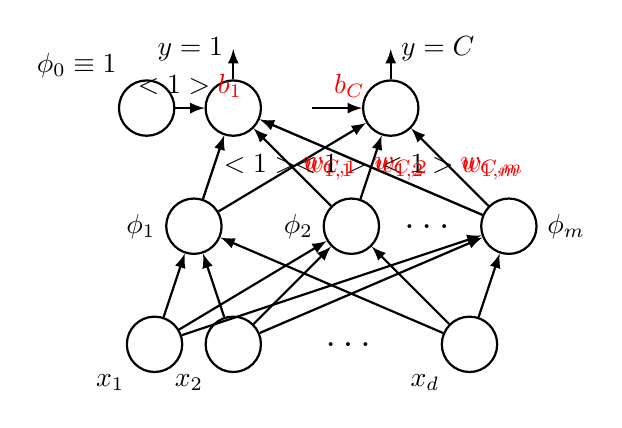
\begin{tikzpicture}
  \node (x1) [cnode,label={below left:$x_1$}] at (0,0) {};
  \node (x2) [cnode,label={below left:$x_2$}] at (1,0) {};
  \node  at (2.5,0) {\Large \ldots};
  \node (xd) [cnode,label={below left:$x_d$}] at (4,0) {};
  \node (phi1) [cnode,label={left:$\phi_1$}] at (.5,1.5) {};
  \node (phi2) [cnode,label={left:$\phi_2$}] at (2.5,1.5) {};
  \node  at (3.5,1.5) {\Large \ldots};
  \node (phim) [cnode,label={right:$\phi_m$}] at (4.5,1.5) {};
  \uncover<1>{\node (phi0) [cnode,label={above left:$\phi_0\equiv 1$}] at  (-.1,3) {};}
  \node (y1) [cnode] at (1,3) {};
  \draw[thick,-latex] (y1)--++(0,.75) node[left] {$y=1$};
  \node (ym) [cnode] at (3,3) {};
  \draw[thick,-latex] (ym)--++(0,.75) node[right] {$y=C$};

  \draw[thick,-latex] (x1)--(phi1);
  \draw[thick,-latex] (x2)--(phi1);
  \draw[thick,-latex] (xd)--(phi1);
  \draw[thick,-latex] (x1)--(phi2);
  \draw[thick,-latex] (x2)--(phi2);
  \draw[thick,-latex] (xd)--(phi2);
  \draw[thick,-latex] (x1)--(phim);
  \draw[thick,-latex] (x2)--(phim);
  \draw[thick,-latex] (xd)--(phim);
  \uncover<1>{
    \draw[thick,-latex] (phi1)--(y1) node [midway,right=-0cm] {$\uncover<1>{\textcolor{red}{w_{1,1}}}$};
    \draw[thick,-latex] (phi2)--(y1) node [midway,right=-0.1cm] {$\uncover<1>{\textcolor{red}{w_{1,2}}}$};
    \draw[thick,-latex] (phim)--(y1) node [midway,right] {$\uncover<1>{\textcolor{red}{w_{1,m}}}$};
    \draw [thick,-latex] (phi0)--(y1) node [midway,above]
    {$\uncover<1>{\textcolor{red}{b_1}}$};
  }
  \uncover<2->{
    \draw[thick,-latex,opacity=.3] (phi1)--(y1);
    \draw[thick,-latex,opacity=.3] (phi2)--(y1);
    \draw[thick,-latex,opacity=.3] (phim)--(y1);
    \draw [thick,-latex,opacity=.3] (phi0)--(y1);
  }
  \uncover<2->{
   \draw[thick,-latex] (phi1)--(ym) node [midway,right=-0cm] {$\textcolor{red}{w_{C,1}}$};
   \draw[thick,-latex] (phi2)--(ym) node [midway,right=-0.1cm] {$\textcolor{red}{w_{C,2}}$};
   \draw[thick,-latex] (phim)--(ym) node [midway,right] {$\textcolor{red}{w_{C,m}}$};
   \draw [thick,-latex] ($(ym)-(1,0)$)--(ym) node [near end,above]
   {$\textcolor{red}{b_C}$};
   }
\end{tikzpicture}
\end{minipage}%

\end{frame}

\begin{frame}
  \frametitle{Two-layer network}
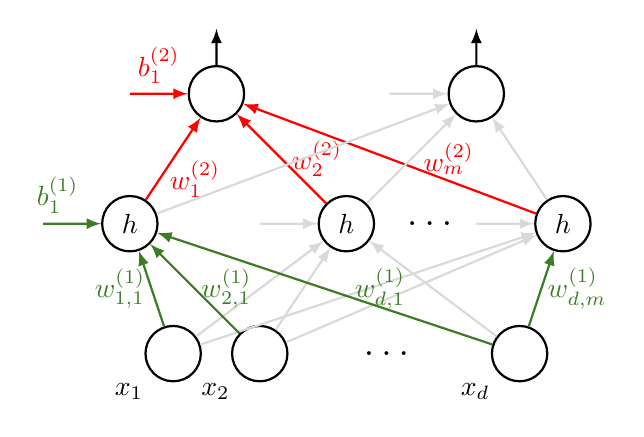
\begin{tikzpicture}[scale=1.1]
  \node (x1) [cnode,label={below left:$x_1$}] at (1,0) {};
  \node (x2) [cnode,label={below left:$x_2$}] at (2,0) {};
  \node  at (3.5,0) {\Large \ldots};
  \node (xd) [cnode,label={below left:$x_d$}] at (5,0) {};
  \node [cnode] (phi1) at (.5,1.5) {$h$};
  \node [cnode] (phi2)  at (3,1.5) {$h$};
  \node  at (4,1.5) {\Large \ldots};
  \node [cnode] (phim) at (5.5,1.5) {$h$};
  \node [cnode](y1) at (1.5,3) {};
  \node [cnode] (yc) at (4.5,3) {};

  \draw[thick,-latex,gray!30] (x1)--(phi2);
  \draw[thick,-latex,gray!30] (x2)--(phi2);
  \draw[thick,-latex,gray!30] (xd)--(phi2);
  \draw[thick,-latex,gray!30] (x1)--(phim);
  \draw[thick,-latex,gray!30] (x2)--(phim);
  \draw[thick,-latex,OliveGreen] (xd)--(phim)
  node[midway,right=-.05cm] {$\textcolor{OliveGreen}{w^{(1)}_{d,m}}$};

  \draw[thick,-latex,OliveGreen] (x1)--(phi1) node [midway,left=-0.05cm] {$\textcolor{OliveGreen}{w_{1,1}^{(1)}}$};
  \draw[thick,-latex,OliveGreen] (x2)--(phi1) node [midway,right=-0.05cm] {$\textcolor{OliveGreen}{w_{2,1}^{(1)}}$};
  \draw[thick,-latex,OliveGreen] (xd)--(phi1) node [midway,right=.25cm] {$\textcolor{OliveGreen}{w_{d,1}^{(1)}}$};
  \draw[thick,-latex,red] (phi1)--(y1) node [near start,right=0cm] {$\textcolor{red}{w_1^{(2)}}$};
  \draw[thick,-latex,red] (phi2)--(y1) node [midway,right=0cm] {$\textcolor{red}{w_2^{(2)}}$};
  \draw[thick,-latex,red] (phim)--(y1) node [midway,right=.3cm] {$\textcolor{red}{w_m^{(2)}}$};
  \draw[thick,-latex,gray!30] (phi1)--(yc);
  \draw[thick,-latex,gray!30] (phi2)--(yc);
  \draw[thick,-latex,gray!30] (phim)--(yc);
  \draw[thick,-latex] (y1)--++(0,.75);
  \draw[thick,-latex] (yc)--++(0,.75);
  \draw [thick,-latex,red] ($(y1)-(1,0)$)--(y1) node [midway,above]
  {$\textcolor{red}{b_1^{(2)}}$};
  \draw [thick,-latex,gray!30] ($(yc)-(1,0)$)--(yc);
  \draw [thick,-latex,gray!30] ($(phi2)-(1,0)$)--(phi2);
  \draw [thick,-latex,gray!30] ($(phim)-(1,0)$)--(phim);
  \draw [thick,-latex,OliveGreen] ($(phi1)-(1,0)$)--(phi1) node [near start,above]
  {$\textcolor{OliveGreen}{b_1^{(1)}}$};
  
\end{tikzpicture}


\bi
\item Idea: learn parametric features
  $\phi_j(\vx)=h(\ip{\textcolor{OliveGreen}{\mathbf{w}^{(1)}_j}}{\vx}+\textcolor{OliveGreen}{b^{(1)}_{j}})$ for some nonlinear function $h$
\ei

\end{frame}


\begin{frame}
  \frametitle{Multilayer perceptrons are universal approximators}
\bi\item Theoretical result [Cybenko, 1989]: 2-layer net with linear
output can approximate any continuous function over compact
domain to arbitrary accuracy (given enough hidden units!)
\item Examples: 3 hidden units with $\tanh(z)=\frac{e^{2z}-1}{e^{2z}+1}$
  activation
\ei
  \begin{tabular}{ccc}
    \includegraphics[width=.26\textwidth]{mlfig/Figure5.3a}&
    \includegraphics[width=.26\textwidth]{mlfig/Figure5.3b}&\\
    \includegraphics[width=.26\textwidth]{mlfig/Figure5.3c}&
    \includegraphics[width=.26\textwidth]{mlfig/Figure5.3d}&{\small [from Bishop]}
  \end{tabular}
\end{frame}


\begin{frame}
  \frametitle{Feed-forward networks}
  \begin{minipage}[c]{.7\linewidth}
\bi
\item Feedforward operation, from input $\vx$ to output $\hat{y}$:
\[f_y(\vx)\;=\;
\sum_{j=1}^m\textcolor{red}{w_{j,y}^{(2)}}h\left(\sum_{i=1}^d
\textcolor{OliveGreen}{w_{i,j}^{(1)}}x_i\,+\,\textcolor{OliveGreen}{b_{j}^{(1)}}
\right)
\,+\,\textcolor{red}{b^{(2)}_y}
\]
\ei
\end{minipage}%
  \begin{minipage}[b]{.3\linewidth}
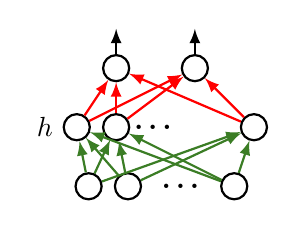
\begin{tikzpicture}[scale=.5]
 \node (x1) [cnodesmall] at (1.3,0) {};
  \node (x2) [cnodesmall] at (2.3,0) {};
  \node  at (3.7,0) {\bf \ldots};
  \node (xd) [cnodesmall] at (5,0) {};

  \node (phi1) [cnodesmall,label={left:$h$}] at (1,1.5) {};
  \node (phi2) [cnodesmall] at (2,1.5) {};
  \node  at (3,1.5) {\bf \ldots};
  \node (phim) [cnodesmall] at (5.5,1.5) {};
  \node (y1) [cnodesmall] at (2,3) {};
  \node (yc) [cnodesmall] at (4,3) {};

  \draw[thick,-latex,OliveGreen] (x1)--(phi2);
  \draw[thick,-latex,OliveGreen] (x2)--(phi2);
  \draw[thick,-latex,OliveGreen] (xd)--(phi2);
  \draw[thick,-latex,OliveGreen] (x1)--(phim);
  \draw[thick,-latex,OliveGreen] (x2)--(phim);
  \draw[thick,-latex,OliveGreen] (xd)--(phim);

  \draw[thick,-latex,OliveGreen] (x1)--(phi1);
  \draw[thick,-latex,OliveGreen] (x2)--(phi1);
  \draw[thick,-latex,OliveGreen] (xd)--(phi1);

  \draw[thick,-latex,red] (phi1)--(y1);
  \draw[thick,-latex,red] (phi2)--(y1);
  \draw[thick,-latex,red] (phim)--(y1);
  \draw[thick,-latex,red] (phi1)--(yc);
  \draw[thick,-latex,red] (phi2)--(yc);
  \draw[thick,-latex,red] (phim)--(yc);

  \draw[thick,-latex] (y1)--++(0,1);
  \draw[thick,-latex] (yc)--++(0,1);
\end{tikzpicture}
\end{minipage}

\bi
\item In matrix form:
\[\mathbf{f}(\vx)\,=\,\ip{\textcolor{red}{\mathbf{W}_2}}
  {h\left(
      \ip{\textcolor{OliveGreen}{\mathbf{W}_1}}{\vx}+\textcolor{OliveGreen}{\mathbf{b}_1}
    \right)}
\,+\,\textcolor{red}{\mathbf{b}_2}
\]
where $h$ is applied elementwise; $\vx\in\mathbb{R}^d$, $\mathbf{W}_1\in\mathbb{R}^{m\times
  d}$, $\mathbf{W}_2\in\mathbb{R}^{C\times m}$,
$\mathbf{b}_2\in\mathbb{R}^C$, $\mathbf{b}_1\in\mathbb{R}^m$
\ei


\end{frame}
 



\begin{frame}
  \frametitle{Learning a neural network}
\begin{align*}
\mathbf{f}(\vx)\,&=\,\ip{\mathbf{W}_2}
  {h\left(
      \ip{\mathbf{W}_1}{\vx}+\mathbf{b}_1
    \right)}
\,+\,\mathbf{b}_2\\
\text{recall:}\:\hat{p}(y=c|\vx)\,&=\,\exp(f_c(\vx))/\sum_j\exp(f_j(\vx))
\end{align*}
  \bi
\item Softmax loss computed on $\mathbf{f}(\vx)$ vs. true label $y$:
\[L(\vx,y)\,=\,-\log\hat{p}(y|\vx)\,=\,-f_y(\vx)+\log\sum_c\exp\left(f_c(\vx)\right)
\]
\item Learning the network: initialize, then run [stochastic] gradient
  descent, updating according to
\[
\frac{\partial L}{\partial \mathbf{w}_2},\quad
\frac{\partial L}{\partial \mathbf{b}_2},\quad
\frac{\partial L}{\partial \mathbf{W}_1},\quad
\frac{\partial L}{\partial \mathbf{b}_1}
\]
\ei
\end{frame}

\begin{frame}
  \frametitle{Chain rule review: vectors}
  \bi
\item Consider the chain (stage-wise) mapping

  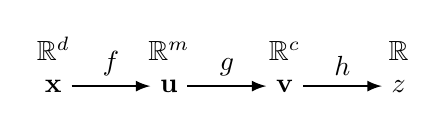
\begin{tikzpicture}
    \node[draw=none,label={above:$\mathbb{R}^d$}] (x) {$\mathbf{x}$};
    \node[draw=none,right=of x,right=1cm,label={above:$\mathbb{R}^m$}] (u) {$\mathbf{u}$};
    \node[draw=none,right=of u,right=1cm,label={above:$\mathbb{R}^c$}] (v) {$\mathbf{v}$};
    \node[draw=none,right=of v,right=1cm,label={above:$\mathbb{R}$}] (z) {$z$};
    \draw[thick,black,-latex] (x)--(u) node[midway,above] {$f$};
    \draw[thick,black,-latex] (u)--(v) node[midway,above] {$g$};
    \draw[thick,black,-latex] (v)--(z) node[midway,above] {$h$};
  \end{tikzpicture}
\item Computing partial gradients:
\[\nabla_{\mathbf{v}}z=\frac{\partial z}{\partial \mathbf{v}}
\]
\uncover<2->{\[\frac{\partial z}{\partial u_i}\,
=\,\sum_j\frac{\partial z}{\partial v_j}
\frac{\partial v_j}{\partial u_i}\;\Rightarrow\;
\nabla_{\mathbf{u}}z\,=\,\left(\frac{\partial \mathbf{v}}{\partial \mathbf{u}}\right)'\nabla_{\mathbf{v}}z
\]
}
\uncover<3->{
  \[\frac{\partial z}{\partial x_k}\,
=\,\sum_q\frac{\partial z}{\partial u_q}
\frac{\partial u_q}{\partial x_k}\;\Rightarrow\;
\nabla_{\mathbf{x}}z\,=\,\left(\frac{\partial \mathbf{u}}{\partial \mathbf{x}}\right)'\nabla_{\mathbf{u}}z
\]
}
\ei
\end{frame}

\begin{frame}
  \frametitle{Chain rule review: tensors}
  \bi
\item More generally, some of the variables are tensors
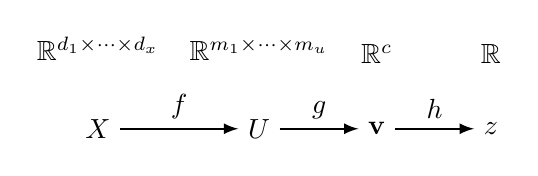
\begin{tikzpicture}
    \node[draw=none,label={[label distance=.5cm]90:$\mathbb{R}^{d_1\times\cdots\times d_x}$}] (x) {$\mathbfsf{X}$};
    \node[draw=none,right=of
    x,right=1.5cm,label={[label distance=.5cm]90:$\mathbb{R}^{m_1\times\cdots\times m_u} $}] (u) {$\mathbfsf{U}$};
    \node[draw=none,right=of u,right=1cm,label={[label distance=.5cm]90:$\mathbb{R}^c$}] (v) {$\mathbf{v}$};
    \node[draw=none,right=of v,right=1cm,label={[label distance=.5cm]90:$\mathbb{R}$}] (z) {$z$};
    \draw[thick,black,-latex] (x)--(u) node[midway,above] {$f$};
    \draw[thick,black,-latex] (u)--(v) node[midway,above] {$g$};
    \draw[thick,black,-latex] (v)--(z) node[midway,above] {$h$};
  \end{tikzpicture}
\item $\nabla_{\mathbfsf{X}}z$ is a tensor, same dim as
  $\mathbfsf{X}$
\item Use single index to indicate index tuples: e.g., if
  $\mathbfsf{X}$ is 3D, $i=(i_1,i_2,i_3)$
\[\left(\nabla_{\mathbfsf{X}}z\right)_i\,=\,
\frac{\partial z}{\partial x_{i_1,i_2,i_3}}
\]
\item Now,
\[\nabla_{\mathbfsf{X}}z\,=\,\sum_j
\left(\nabla_{\mathbfsf{X}}\mathbfsf{U}_j\right)
\left(\nabla_{\mathbfsf{U}}z\right)_j
\]
\ei
\end{frame}

\begin{frame}
  \frametitle{Staged feedforward computation}
\bi
\item To make derivations more convenient, we will express forward
  computation $(\vx,y)\,\to\,L$ in more detail:
\begin{align*}
\vx,\,\mathbf{W}_1,\mathbf{b}_1\,&\to\,\mathbf{a}_1\,=&\,\ip{\mathbf{W}_1}{\vx}+\mathbf{b}_1\\
\mathbf{a}_1\,&\to\,\mathbf{z}_1\,=&\,h(\mathbf{a}_1)\\
\mathbf{z}_1,\,\mathbf{W}_2,\mathbf{b}_2\,&\to\,\mathbf{a}_2\,=&\ip{\mathbf{W}_2}{\mathbf{z}_1}+\mathbf{b}_2\\
\mathbf{a}_2,\,y\,&\to\,L\,=&\,-\ip{\mathbf{e}_y}{\mathbf{a}_2}\,+\,
       \log \left[\ip{\mathbf{1}}{\exp(\mathbf{a}_2)}\right]\\
\end{align*}
\vspace{-2em}
\item Now we have, e.g.,
\uncover<2->{
\[\nabla_{\mathbf{z}_1}L\,=\,\left(\frac{\partial
      \mathbf{a}_2}{\partial \mathbf{z}_1}\right)'\nabla_{\mathbf{a}_2}L,
\]}
\uncover<3->{
\[
\nabla_{\mathbf{W}_1}L\,=\,\sum_j\left(\nabla_{\mathbf{W}_1}z_{1,j}\right)
\left(\nabla_{\mathbf{z}_1}L\right)_j
\]
}
\item What is $\nabla_{\mathbf{W}_1}z_{1,j}$ like?
\ei
\end{frame}

\section{Backpropagation}



\begin{frame}
  \frametitle{Backpropagation: general network}
  \bi\item General unit activation in a network (ignoring bias)
\item Unit $t$ receives input from $I(t)=\{i_1,\ldots,i_S\}$, sends to $O(t)=\{o_1,\ldots,o_R\}$
\ei
\begin{minipage}[c]{.55\linewidth}
  \begin{align*}
a_t\;&=\;\sum_{j\in I(t)}w_{jt}z_j\\
z_t\,&=\,h(a_t)
\end{align*}
\bi
\item The loss $L$ depends on $w_{jt}$ only through $a_t$
\begin{align*}
\frac{\partial L}{\partial w_{jt}}\;&=\;
\frac{\partial L}{\partial a_t}
\frac{\partial a_t}{\partial w_{jt}}
\\
\uncover<2->{
&=\;\frac{\partial L}{\partial a_t}z_j
}
\end{align*}
\ei
\end{minipage}%
\begin{minipage}[c]{.45\linewidth}
\raisebox{2em}{  \tikz[scale=.8]{
    \node [cnode] (a) at (1.75,1.5) {$z_t$};
    \node [cnode] (z1) at (0,0) {$z_{i_1}$};
    \draw [thick,-latex,ffcol] (z1)--(a) node [midway,left] {$w_{i_1,t}$};
    \node [cnode] (z2) at (1.25,0) {$z_{i_2}$};
    \draw [thick,-latex,ffcol] (z2)--(a) node [midway,right] {$w_{i_2,t}$};
    \node at (2.5,0) {\Large \ldots};
    \node [cnode] (zs) at (3.75,0) {$z_{i_S}$};
    \draw [thick,-latex,ffcol] (zs)--(a) node [midway,right] {$w_{i_S,t}$};
    \node [cnode] (zt+1) at (0.5,3) {$z_{o_1}$};
    \node [draw=none] at (2,3) {\Large \ldots};
    \node [cnode] (zT) at (3.25,3) {$z_{o_R}$};
    \draw [thick,-latex,ffcol] (a)--++(zt+1) node [midway,left] {$w_{t,o_1}$};
    \draw [thick,-latex,ffcol] (a)--++(zT) node [midway,right] {$w_{t,o_R}$};
    
    \node[cnode] (f1) at (1,6) {$f_1$};
    \node at (2,6) {\Large \ldots};
    \node[cnode] (fC) at (3,6) {$f_C$};
    \node[draw=none] (L) at (2,6.8) {$L$};
    \draw[thick,-latex,ffcol] (f1)--(L);
    \draw[thick,-latex,ffcol] (fC)--(L);
    
    \node [draw=none] at (2,4.5) {\Huge \ldots};

    \convarr[ffcol]{f1}{-1}
    \convarr[ffcol]{fC}{-1}
    
    \divarr[ffcol]{zt+1}{1};
    \divarr[ffcol]{zT}{1};

  }}
\end{minipage}

\end{frame}


\begin{frame}
  \frametitle{Backpropagation: general network}
  \begin{minipage}[c]{.55\linewidth}
    \bi
  \item Starting with $L$, compute backward (gradient) flow
  \item Note: 
    \begin{align*}
      a_{j}=\sum_{i\in I(j)}w_{i,j}h(a_i)
    \end{align*}
    \vspace{-1em}
  \item Notation: $d_t=\frac{\partial L}{\partial a_t}$
  \item The backward flow comes to unit $t$ from $O(t)$:
    \begin{align*}
      d_t\,
      &=\,\sum_{o\in O(t)}\textcolor{red}{\frac{\partial L}{\partial a_o}}
        \frac{\partial a_o}{\partial a_t}
      \\
      &=\,\sum_{o\in O(t)}d_ow_{t,o}h'(a_t)\uncover<2->{
        \,=\,h'(a_t)\sum_{o\in O(t)}d_ow_{t,jo}
        }
    \end{align*}
\ei
  \end{minipage}%
  \begin{minipage}[c]{.45\linewidth}
    \raisebox{3em}{\tikz[scale=.8]{
    \node [cnode] (a) at (1.75,1.5) {$z_t$};
    \node [cnode] (z1) at (0,0) {$z_{i_1}$};
    \draw [thick,latex-,bpcol] (z1)--(a) node [midway,left] {$w_{i_1,t}$};
    \node [cnode] (z2) at (1.25,0) {$z_{i_2}$};
    \draw [thick,latex-,bpcol] (z2)--(a) node [midway,right] {$w_{i_2,t}$};
    \node at (2.5,0) {\Large \ldots};
    \node [cnode] (zs) at (3.75,0) {$z_{i_S}$};
    \draw [thick,latex-,bpcol] (zs)--(a) node [midway,right] {$w_{i_S,t}$};
    \node [cnode] (zt+1) at (0.5,3) {$z_{o_1}$};
    \node [draw=none] at (2,3) {\Large \ldots};
    \node [cnode] (zT) at (3.25,3) {$z_{o_R}$};
    \draw [thick,latex-,bpcol] (a)--++(zt+1) node [midway,left] {$w_{t,o_1}$};
    \draw [thick,latex-,bpcol] (a)--++(zT) node [midway,right] {$w_{t,o_R}$};
    
    \node[cnode] (f1) at (1,6) {$f_1$};
    \node at (2,6) {\Large \ldots};
    \node[cnode] (fC) at (3,6) {$f_C$};
    \node[draw=none] (L) at (2,6.8) {$L$};
    \draw[thick,latex-,bpcol] (f1)--(L);
    \draw[thick,latex-,bpcol] (fC)--(L);
    
    \node [draw=none] at (2,4.5) {\Huge \ldots};

    \divarr[bpcol]{f1}{-1};
    \divarr[bpcol]{fC}{-1};

    \convarr[bpcol]{zt+1}{1};
    \convarr[bpcol]{zT}{1};

  }}
  \end{minipage}
\end{frame}

\begin{frame}
  \frametitle{Multilayer networks}
  \bi
\item Consider a layer $t$ with $n_t$ units
\[\mathbf{z}_t\,=\,h\left(\mathbf{W}_t\mathbf{z}_{t-1}+\mathbf{b}_t\right)
\]
where $\mathbf{z}_t\in\mathbb{R}^{n_t}$, $\mathbf{b}_t\in\mathbb{R}^{n_t}$,
$\mathbf{W}_{t}\in\mathbb{R}^{n_{t}\times n_{t-1}}$ \\
$h$ is applied element-wise
\item Layer zero reads off input $\mathbf{z}_0\,\equiv\,\mathbf{x}$
\item Last layer $T$ produces a linear output
\[\mathbf{z}_T\,=\,\mathbf{W}_T\mathbf{z}_{T-1}+\mathbf{b}_T\]
which is used to predict/assess loss (a.k.a. $\mathbf{f}$)
\ei
\end{frame}

\begin{frame}
  \frametitle{Feed-forward pass}
  \bi
\item Compute 
  \begin{align*}
    \mathbf{a}_1 & =\ip{\mathbf{W}_1}{\vx}+\mathbf{b}_1&\mathbf{z}_1&=h(\mathbf{a}_1)\\
    \uncover<2->{
    \mathbf{a}_2 & =\ip{\mathbf{W}_2}{\mathbf{z}_1}+\mathbf{b}_2&\mathbf{z}_2&=h(\mathbf{a}_2)\\
    }
    \uncover<3->{
    \ldots\\
    \mathbf{a}_{T-1} & =\ip{\mathbf{W}_{T-1}}{\mathbf{z}_{T-2}}+\mathbf{b}_{T-1}&\mathbf{z}_{T-1}&=h(\mathbf{a}_{T-1})\\
    }
    \uncover<4->{
    \mathbf{a}_{T} & =\ip{\mathbf{W}_{T}}{\mathbf{z}_{T-1}}+\mathbf{b}_{T}&\mathbf{z}_{T}&=\mathbf{a}_{T}\\
    }
  \end{align*}



\item<4-> Training: Compute $L(\mathbf{z}_T,y)$
\item<4-> Testing: make inference 
  \[
    \hat{y}(\vx)\,=\,\argmax_c z_{T,c}
  \]
\ei
\end{frame}


\begin{frame}
  \frametitle{Backward pass}
  \bi
\item The main backprop equations:
\[d_t\,=\,h'(a_t)\sum_{j\in O(t)}d_jw_{t,j},\qquad
  \frac{\partial L}{\partial w_{i,t}}\,=\,d_tz_i
\]

\item Compute gradient information, using cached $\mathbf{z}$ and $\mathbf{a}$
  \begin{align*}
  \mathbf{d}_T\,
    &=\,\frac{\partial L}{\mathbf{a}_T}
    &\nabla_{\mathbf{W}_T}L\,
    &=\,\mathbf{d}_T\otimes\mathbf{z}_{T-1}\;
    \\
    \uncover<2->{
    \mathbf{d}_{T-1}\,
    &=\,h'(\mathbf{a}_{T-1})\ast\left(\mathbf{d}_T'\mathbf{W}_T\right)
    &\nabla_{\mathbf{W}_{T-1}}L\,
    &=\,\mathbf{d}_{T-1}\otimes\mathbf{z}_{T-2}\\
    }
    \uncover<3->{
    &\ldots&&\\
     \mathbf{d}_{t}\,
    &=\,h'(\mathbf{a}_{t})\ast\left(\mathbf{d}_{t+1}'\mathbf{W}_{t+1}\right)
    &\nabla_{\mathbf{W}_{t}}L\,
    &=\,\mathbf{d}_{t}\otimes\mathbf{z}_{t-1}\\
    }
  \end{align*}
\item $\mathbf{u}\otimes\mathbf{v}$: outer prod;
  \uncover<2->{$\mathbf{u}\ast\mathbf{v}$: elt-wise}
\ei
\end{frame}



\begin{frame}
  \frametitle{Modularity}
  \bi
\item Basic building block of a neural network: a layer, which defines
  two directions of computation
\item Forward: pull activations from input units;\\ 
compute and cache ``raw'' activation $\mathbf{a}$;\\
compute and output activation $\mathbf{z}=h(\mathbf{a})$
\item Backward: collect gradient information $\mathbf{d}$ from output
  units;\\
calculate gradient w.r.t. $\mathbf{a}$;\\
calculate gradient w.r.t. weights and biases
\item The only connections between layers is in communicating
  $\mathbf{z}$ and $\mathbf{d}$
\ei
\end{frame}

\begin{frame}
  \frametitle{Computational graph}
  \bi
\item When implementing backpropagation, existing software falls into
  two groups
\item Numerical: interface between layers handles numbers; computation
  must be fully specified\\
Torch,MatConvnet,Caffe
\ei
  \begin{minipage}[c]{.5\linewidth}
\bi
\item Symbolic: interface includes derivatives (and
  intermediate stages) as first-class citizens. Computation is
  specified by a computational graph\\
Theano, TensorFlow, Caffe2
   
\ei
  \end{minipage}%
  \begin{minipage}[c]{.5\linewidth}
\includegraphics[width=.95\textwidth]{gcb-compgraph-example}

[Goodfellow et al]    
  \end{minipage}





\end{frame}


\section{Activation functions}
\begin{frame}
  \frametitle{Choice of non-linearity: 1070s-2010}
\begin{minipage}[c]{.5\linewidth}
\[\text{sigmoid}:\:[h(a)\,=\,\frac{1}{1+\exp(a)}
\]
\includegraphics[width=.7\textwidth]{ak-sigmoid}

\end{minipage}%
\begin{minipage}[c]{.5\linewidth}
\[h(a)\,=\,\tanh(a)
\]
\includegraphics[width=.7\textwidth]{ak-tanh}

\end{minipage}

\bi
\item Good: squash activations to a fixed range
\item Bad: gradient is nearly zero far away from midpoint
\[\frac{\partial L}{\partial a}\,=\,\frac{\partial L}{\partial h(a)}
\textcolor{red}{\frac{d h}{d a}}\,\approx\,0
\]
can make learning very, very slow
\item $\tanh$ (zero-centered) is preferable to sigmoid 
\ei
\end{frame}


\begin{frame}
  \frametitle{2010: RELU}
  \bi
\item Intuition: make the non-linearity non-saturating, at least in
  part of the range
\ei
\begin{minipage}[c]{.5\linewidth}
\bi  \item Rectified linear units: 
\[h(a)=\max(0,a)\]
\ei
\end{minipage}%
\begin{minipage}[c]{.5\linewidth}
  \includegraphics[width=.75\textwidth]{ak-relu}
\end{minipage}
\bi
\item Good: non-saturating; cheap to compute; \\
greatly speeds up convergence compared to sigmoid (order of magnitude)
\ei
\end{frame}
\begin{frame}
  \frametitle{RELU and dead units}
  \bi
\item Problem: if RELU gets into a state in which all batches in an
  epoch have zero activation, the units becomes stuck with
  zero gradient (``dies'').

\includegraphics[width=.7\textwidth]{ak-deadrelus} [A. Karpathy]

\ei
\end{frame}

\begin{frame}
  \frametitle{RELU variants}
  \bi
\item Many attempts to improve RELUs:
\ei
\begin{minipage}[c]{.55\linewidth}
\bi
\item  Leaky RELU: $h(a)=max(\alpha a, a)$
\item Learning $\alpha$: Parametric RELU
\item Exponential RELUs:
\[h(a)=
  \begin{cases}
    a & \text{if}\;a\ge 0,\\
    \alpha(\exp(a)-1) &\text{if}\;a<0
  \end{cases}
\]
\ei
\end{minipage}%
\begin{minipage}[c]{.45\linewidth}
  \includegraphics[width=.97\textwidth]{ak-activations} 

~~[A. Karpathy]
\end{minipage}

\bi
\item ELU are promising, but more expensive to compute
\item RELU still the default choice;\\
none of the variants are consistently better
\ei
\end{frame}



\section{Initialization}

\begin{frame}
  \frametitle{Random initialization}
  \bi
\item Non-convex objective; initialization is important
\item Can we initialize with all zeros?\\
bad idea: all units will learn the same thing!
\item Can initialize weights with small real numbers, e.g., drawn from
  Gaussian with zero mean, variance 0.01
\item Problem: variance of activation grows with number of inputs

\includegraphics[width=.6\textwidth]{ak-layer-stats-random-init}

[A. Karpathy]
\ei
\end{frame}

\begin{frame}
  \frametitle{Xavier initialization}
  \bi
\item Idea: normalize the scale to provide roughly equal variance
  throughout the network
\item the \texttt{Xavier} initialization [Glorot et al]: if unit has
  $n$ inputs, draw from zero mean, variance $1/n$

\includegraphics[width=.6\textwidth]{ak-layer-stats-xavier-init}

[A. Karpathy]
\ei
\end{frame}


\begin{frame}
  \frametitle{Initialization and RELU}
  \bi
\item Assumption behind Xavier: (1) linear activations, (2) zero mean
  activations. 
\item Breaks when using RELUs:

\includegraphics[width=.6\textwidth]{ak-layer-stats-xavier-init-relu}

[A. Karpathy]
\ei
\end{frame}

\begin{frame}
  \frametitle{Kaiming initialization}
  \bi
\item Initialization scheme specifically for RELUs [He et al.]:\\
zero mean, variance $2/n$ where $n$ is the number of inputs.
\item The \texttt{Kaiming} initialization currently recommended for
  RELU units

\includegraphics[width=.6\textwidth]{ak-layer-stats-kaiming-init}

[A. Karpathy]
\item Note: still OK to init biases with zeros
\ei
\end{frame}

\section{Optimization tricks}

\begin{frame}
  \frametitle{Basic stochastic gradient descent}
  \bi
\item Learning hyperparameters: architecture, regularizer $R$
\item Hyperparameters: learning rate $\eta$, batch size $B$
\item Initialize weights and biases
\item Each epoch: shuffle data, partition into batches, iterate over
  batches $b$
\[\mathbf{w}\,=\,\mathbf{w}-\eta\left[
    \nabla_{\mathbf{w}}L(X_b,Y_b)\,+\,\nabla_{\mathbf{w}}R(\mathbf{w})
\right]
\]
\item We have covered initialization
\item Next: optimization
\ei
\end{frame}


\begin{frame}
  \frametitle{Learning rate}
  \bi
\item Generally, for convex functions, gradient descent will converge
\item Setting the learning rate $\eta$ may be very important to ensure
  rapid convergence
  \begin{minipage}[c]{.6\linewidth}
\includegraphics[height=.7\textheight]{mlfig/etaplots}
  \end{minipage}%
  \begin{minipage}[c]{.4\linewidth}
from Lecun et al, 1996        
  \end{minipage}

\ei
\end{frame}


\begin{frame}
  \frametitle{Learning rate for neural networks}
  \bi
\item For deep networks, setting the right learning rate is crucial.
\item Typical behaviors, monitoring \emph{training loss}:
\includegraphics[width=.5\textwidth]{lrates-karpathy}[A. Karpathy]
\ei
\end{frame}

\begin{frame}
  \frametitle{Learning rate schedules}
  \bi
\item Generally, as with convex functions, we want the learning rate
  to decay with time
\item Could set up automatic schedule, e.g., drop by a factor of
  $alpha$ every $\beta$ epochs.
\item Most common in practice: some degree of babysitting\\
start with a resonable learning rate\\
monitor training loss\\
drop LR (typically 1/10) when learning appears stuck
\ei
\end{frame}

\begin{frame}
  \frametitle{Monitoring training loss}
  \begin{minipage}[c]{.6\linewidth}
  \bi
\item Too expensive to evaluate on entire training set frequently;
  instead, use rolling average of batch loss value
\item Typical behavior: the red line
\ei    
  \end{minipage}%
  \begin{minipage}[c]{.4\linewidth}\begin{center}
    \includegraphics[width=.97\textwidth]{lr-drops-plot-fractalnet}\\
 ~[Larsson et al.]\end{center}
  \end{minipage}
\bi
\item A few caveats:\\
wait a bit before dropping;\\
remember that this is surrogate loss on training (monitor validation
accuracy as a precaution)\\
better yet, drop LR based on val accuracy, not training loss\\
do a sanity check for loss values
\item Crashes due to NaNs etc. often due to high LR
\ei
\end{frame}


  \begin{frame}
   \frametitle{Gradient Descent with Momentum}
 \bi
 \item SGD(GD) has trouble navigating ravines, i.e. areas where the
   surface curves much more steeply in one dimension than in another,
   which are common around local optima. 
\includegraphics[width=.8\textwidth]{ravine-karpathy}

[A. Karpathy]
\item SGD oscillates across the slopes of the ravine, only making hesitant progress towards the local optimum.
 \item Momentum is a method that helps accelerate SGD(GD) in the relevant direction and dampens oscillations.
 \pause
 \begin{align*}
 \Delta w_{t} &= \gamma \Delta w_{t-1} + \eta _t \nabla f(w_t)\\
 w_{t+1} &= w_t - \Delta w_{t}
 \end{align*}
 \ei
 \end{frame}

      \begin{frame}
   \frametitle{Gradient Descent with Momentum}
 \bi
 \item Essentially, when using momentum, we push a ball down a hill. The ball accumulates momentum as it rolls downhill, becoming faster and faster on the way (until it reaches its terminal velocity if there is air resistance, i.e. $\gamma < 1$). 
 \pause
 \item The momentum term increases for dimensions whose gradients
   point in the same directions, reduces updates for dimensions whose
   gradients change directions. 
\ei
\begin{minipage}[c]{.6\linewidth}
\bi
\item Faster convergence, reduced oscillation  
\ei
\end{minipage}%
\begin{minipage}[c]{.4\linewidth}
  \includegraphics[width=0.8\textwidth]{gcb-sgd-momentum}

[Goodfellow et al]

\end{minipage}
 \end{frame}


 \begin{frame}
   \frametitle{AdaGrad}
\bi
\item Intuition [Duchi et al.]: parameters (directions of the parameter space)
  are updated with varying frequency
\item Idea: reduce learning rate in proportion to the updates
\item Maintain cache $s_i$ for each parameter $\theta_i$; when updating,
\begin{align*}
s_i\,&=\,s_i\,+\,\left(\frac{\partial L}{\partial \theta_i}\right)^2\\
w_i\,&=\,w_i-\eta \frac{\partial L}{\partial \theta_i}\,/\,
\left(\sqrt{s_i}\,+\,\epsilon\right)
\end{align*}
\item Rarely used today (reduces rate too aggresively)
\ei
 \end{frame}

 \begin{frame}
   \frametitle{RMSprop}
   \bi
\item Modified idea from Adagrad; `[``published'' in Hinton's Coursera
  slides]
\item Cached rate allows for ``forgetting''
  \begin{align*}
    s_i\,&=\,\delta s_i\,+\,(1-\delta)\left(\frac{\partial L}{\partial
           \theta_i}\right)^2,\\
    w_i\,&=\,w_i-\eta \frac{\partial L}{\partial \theta_i}\,/\,
\left(\sqrt{s_i}\,+\,\epsilon\right)
  \end{align*}
\item The decay rate $\delta$ is typically 0.9--0.99
\ei
 \end{frame}

 \begin{frame}
   \frametitle{Adam optimizer}
\bi
\item Kind of like RMSprop with momentum [Kingma et al.]
\item First order momentum update for $w_i$:
\[m_i\,=\,\beta_1m_i\,+\,(1-\beta_1)\frac{\partial L}{\partial \theta_i}
\]
\item Second order:
\[v_i\,=\,\beta_2v_i\,+\,(1-\beta_2)\left(\frac{\partial L}{\partial \theta_i}\right)^2
\]
\item Parameter update:
\[w_i\,=\,w_i-\eta \frac{m}{\sqrt{v}\,+\,\epsilon}
\]
\ei
   
 \end{frame}





\begin{frame}
  \frametitle{Warm start}
  \bi
\item Suppose we want to continue training network for more epochs
\item All significant platforms allow for saving snapshots and
  resuming
\item Need to be careful with learning rate: if re-initialize to high,
  might lose our place in parameter space
\item Technical issues with momentum, Adam etc. -- need to save
  relevant data in the snapshots to resume!
\ei
\end{frame}


\section{Regularization}

\begin{frame}
  \frametitle{Review: regularization}
  \bi
\item Main challenge in machine learning: overfitting
\item Bias-variance tradeoff:\\
complex models reduce bias (approximation error), but increase
variance (estimation error)
\item Optimization error: source of concern when dealing with
  non-convex models
\item Bayes error: presumed low in vision tasks (?)
\ei
\end{frame}


\begin{frame}
  \frametitle{Review: regularization}
\bi
\item Regularization as a way to control the bias-variance tradeoff
\item General form of regularized ERM for model class $\mathcal{M}$:
\[\min_{M\in\mathcal{M}}\,\left\{ \sum_i L(y_i,M(\vx_i))\,+\,\lambda R(M)
\right\}
\]
\item For parametric models, choice of $M$ determined by setting value
  to some $\mathbf{w}\in\mathbb{R}^D$
\item Most common form of regularizer $R$: norm $\sum_d|w_d|^p$ \\
(shrinkage)
\ei  
\end{frame}


\begin{frame}
  \frametitle{Review: geometry of regularization}
  \bi
\item Can write unconstrained optimization problem
\[\min_{\mathbf{w}}\sum_{i=1}^N-\log\hat{p}(y_i|\vx_i;\mathbf{w})\,+\,\textcolor{red}{\lambda}\sum_{j=1}^m|w_j|^p
\] 
as an equivalent constrained problem
\ei
\begin{minipage}[c]{.45\textwidth}

\begin{align*}
  \min_{\mathbf{w}}\sum_{i=1}^N&-\log\hat{p}(y_i|\vx_i;\mathbf{w})\\
  \text{subject to}\;&\sum_{j=1}^m|w_j|^p\,\textcolor{red}{\le\,t}
\end{align*}
\end{minipage}%
\begin{minipage}[c]{.55\textwidth}
%\multiinclude[graphics={width=.99\textwidth}]{mlfig/errgeom}
\includegraphics[width=.99\textwidth]{mlfig/errgeom}
\end{minipage}

\bi
 \item<1-> $p=1$ may lead to sparsity, $p=2$ generally won't
\ei

\end{frame}


\begin{frame}
  \frametitle{Effect of regularization}
  
\bi
\item Cartoon of the effect of regularization on bias and variance:

\hspace{-1em}\includegraphics[width=.8\textwidth]{mlfig/Figure3.6} [Bishop]
\item In practice, curves are less clean
\ei

\end{frame}

\begin{frame}
  \frametitle{Weight decay}
  \bi
\item In neural networks, $L_2$ regularization is called weight decay
\item Note: bias is normally not regularized
\item Easy to incorporate weight decay into the gradient calculation
\[\nabla_{\mathbf{w}}\lambda\|\mathbf{w}\|^2\,=\,2\lambda\mathbf{w}
\]
\item One more hyperparameter $\lambda $to tune\\
with large data sets, typically seems inconsequential
\ei
\end{frame}

\begin{frame}
  \frametitle{Dropout}
  \bi
\item Part of overfitting in a neural net: unit co-adaptation\\
idea: prevent it by disrupting co-firing patterns
\item Dropout [Srivastava et al]: during each training iteration,
  randomly ``remove''  units, just for that update 

\includegraphics[width=.7\textwidth]{dropout-ill}
\ei

\end{frame}


\begin{frame}
  \frametitle{Dropout as regularizer}
  \bi
\item With each particular dropout set, we have a different network
\item Interpretation: training an ensemble of networks with shared
  parameters

\includegraphics[width=.55\textwidth]{gcb-dropout-ensemble} \raisebox{3em}{[Goodfellow et al.]}
\ei
\end{frame}

\begin{frame}
  \frametitle{Dropout: implementation}
  \bi
\item Dropout introduces a discrepancy between train and test
\item Correction: suppose survival rate of a unit is $p$\\
must scale weights from unit (after training) by $p$
\item Modern version: ``inverse dropout''\\
scale activations by $1/p$ during training,\\
do not scale during test
\item Typically employed in top layers; $p=0.5$ is most common
\ei
\end{frame}

\section{Convolutional networks}

\begin{frame}
  \frametitle{Sparse weight patterns}
  \bi
\item One way to regularize is to sparsify parameters
\item We can set a subset of weights to zero
\item If the input has ``spatial'' semantics: can keep only weights
  for a contiguous set of inputs
\ei

\begin{tabular}[c]{cc}
  \includegraphics[width=.48\textwidth]{gcb-densenet-above-ill} &
  \includegraphics[width=.48\textwidth]{gcb-sparsenet-above-ill}
\end{tabular}
[Goodfellow et al.]

\end{frame}


\begin{frame}
  \frametitle{Receptive field}
  \bi
\item Each unit in upper layer is affected only by a subset of units
  in lower layer  -- its \emph{receptive field}
\ei

\begin{tabular}[c]{cc}
  \includegraphics[width=.48\textwidth]{gcb-densenet-ill} &
  \includegraphics[width=.48\textwidth]{gcb-sparsenet-above-ill}
\end{tabular}
[Goodfellow et al.]
\bi
\item Conversely: each unit in lower layer only influences a subset of
  units in upper layer
\ei
\end{frame}

\begin{frame}
  \frametitle{Receptive field growth}
  \bi
\item Very important: receptive field size w.r.t. the \emph{input} in locally connected
  networks grows with layers, even if in each layer it is fixed
\ei

\includegraphics[width=.48\textwidth]{gcb-rf-ill}

[Goodfellow et al.]
\end{frame}

\begin{frame}
  \frametitle{Locally connected + parameter sharing}
  \bi
\item We can further reduce network complexity by \emph{tying} weights
  for all receptive fields in a layer
\ei
  \begin{tabular}{cc}
    not tied & tied\\
    \includegraphics[width=.48\textwidth]{gcb-locallyconn}&
    \includegraphics[width=.48\textwidth]{gcb-convconn}\\
Goodfellow et al. &
  \end{tabular}
\bi
\item We have now introduced \emph{convolutional} layers\\
weight sharing induces equivariance to translation!
\ei
\end{frame}

\begin{frame}
  \frametitle{2D convolutions}
  \begin{minipage}[c]{.25\linewidth}
    \bi
\item Note: filters are not flipped
\ei
  \end{minipage}%
  \begin{minipage}[c]{.75\linewidth}
\includegraphics[width=.9\textwidth]{gcb-conv2dexample}

[Goodfellow et al.]    
  \end{minipage}


\end{frame}


\begin{frame}
  \frametitle{Convolutional layer operation}
  \bi
\item Suppose the input to the layer (output of previous layer) has
  $C$ channels\\
tensor $W\times H\times C$
\item we convolve only along spatial dimensions: assuming {\tt valid}
  convolution, with $k\times k\times C$ filter (must match
  \#channels!) we get $(W-k+1)\times(H-k+1)\times 1$ activation map

\includegraphics[width=.7\textwidth]{ak-conv-2maps-ill}
\raisebox{2em}{[A. Karpathy]}
\item If we have $m$ filters, we get $(W-k+1)\times(H-k+1)\times m$
  map as the output of the layer
\ei
\end{frame}

\begin{frame}
  \frametitle{Implementation: efficient convolutions}
  \bi
\item Most common: convert convolution into matrix multiplication\\
parallel, GPU-friendly!
\item Suppose we have $m$ filters $\mathbf{k}_1,\ldots,\mathbf{k}_m$ of size $f\times f$, with
  $c$ channels.
\item Basic idea: pre-compute index mapping 
\[\texttt{im2col}:\mathbfsf{Z}\in\mathbb{R}^{S\times S\times
  c}\to\mathbf{M}\in\mathbb{R}^{(S-f+1)^2\times k^2c}\]
that maps every receptive field to a column in $\mathbf{M}$
\item Collect filters as columns of $\mathbf{K}\in\mathbb{R}^{f^2c}$
\item Now simply compute $\mathbf{M}\mathbf{K}+\mathbf{b}$ and reshape to
  $(S-f+1)\times (S-f+1)\times m$
\item Notably, for some cases (in particular small filters, $3\times
  3$ or $5\times 5$) more efficient implementations use FFT
\item Most software uses 3rd party (Nvidia, Nervana) implementations
  under the hood
\ei
\end{frame}


\begin{frame}
  \frametitle{Conv layer sizing}
\bi
\item If we simplye rely on {\tt valid} convolutions, the maps will
  quickly shrink

\includegraphics[width=.4\textwidth]{gcb-conv-nopad}\raisebox{1em}{[Goodfellow
et al]}

\item Instead, we usually \emph{pad} with zeros

\includegraphics[width=.5\textwidth]{gcb-conv-pad}\raisebox{1em}{[Goodfellow
et al]}
\item Usual padding is symmetric, with $(f-1)/2$ -- {\tt same}
  convolution in Matlab speak
\ei  
\end{frame}

\begin{frame}
  \frametitle{Convolution size}
  \bi
\item Two extreme cases:
\item Filter size equal to output map size of the previous layer\\
\myar fully connected layer (more on this later)
\item Filter size is $1\times1$\\
\myar The layer simply computes a (non-linear) projection of the features
computed by previous layer

\includegraphics[width=.6\textwidth]{ak-1x1conv}\raisebox{1em}{A. Karpathy}
\ei
\end{frame}



\begin{frame}
  \frametitle{Stride and size}
  \bi
\item Convolution with stride \textgreater 1 is a cheap way to reduce
  spatial dimension of output
\item Can be implemented as convolution followed by downsampling
  \begin{minipage}[c]{.4\linewidth}
    \includegraphics[width=.9\textwidth]{gcb-downconv}
  \end{minipage}%
  \begin{minipage}[c]{.5\linewidth}
    used in LeNet\\
    wasteful!\\
    Goodfellow et al.
  \end{minipage}

\item Modern implementations explicitly specify stride

    \includegraphics[width=.4\textwidth]{gcb-strideconv}\raisebox{1em}{[Goodfellow
et al]}
\item Note: matches the multiplication implementation of conv well!
\ei
\end{frame}



\begin{frame}
  \frametitle{Pooling}
  \bi
\item Pooling applies a non-parameterized operation on a receptive
  field
\item Most common operation: max and average
\ei
\begin{minipage}[c]{.5\linewidth}
\bi
\item Typically, pooling is applied with a stride\textgreater 1, to
  reduce spatial resolution

\ei  
\end{minipage}%
\begin{minipage}[c]{.5\linewidth}
  \includegraphics[width=.95\textwidth]{pooling}
\end{minipage}
\bi
\item but is possible to have stride of 1!
\ei
\end{frame}

\begin{frame}
  \frametitle{Maxout pooling}
  \bi
\item Idea: pool over \emph{feature channels}, not spatially
\item Introduces invariance w.r.t. a family of filters

\includegraphics[width=.6\textwidth]{gcb-maxout}~\raisebox{1em}{[Goodfellow
  et al.]}

\ei

\end{frame}

\begin{frame}
  \frametitle{Invariances learned by the network}
  \bi
\item Invariance to translations: due to pooling
\item As we stack layers; invariance to deformations
\item Invariance to lighting: if we normalize input
\item Invariance to rotations? only as present in data
\item Invariance to scale? ditto
\ei
\end{frame}

\begin{frame}
  \frametitle{Case study: LeNet}
\includegraphics[width=.9\textwidth]{lenet}
\bi
\item LeCun et al., 1986
\ei

\end{frame}

\begin{frame}
  \frametitle{AlexNet}
  \includegraphics[width=.9\textwidth]{alexnet}
\bi
\item Krizhevsky et al., 2012
\ei
\end{frame}




\begin{frame}
  \frametitle{VGG-16}
  \begin{minipage}[c]{.5\linewidth}
  \bi
\item Simonyan and Zisserman, 2014
\ei

\includegraphics[width=.9\textwidth]{vgg16}\\
~[{\tt blog.heuritech.com}]
  \end{minipage}%
  \begin{minipage}[c]{.5\linewidth}
    \includegraphics[width=.9\textwidth]{vgg16-table}    
  \end{minipage}

\end{frame}

\begin{frame}
  \frametitle{Visualization}
  \bi
\item Retrieving maximally inducing receptive fields [Girshick et al]:
\ei
\includegraphics[width=.99\textwidth]{pool5max}
\end{frame}


\end{document}
